\begin{figure}
    \centering
    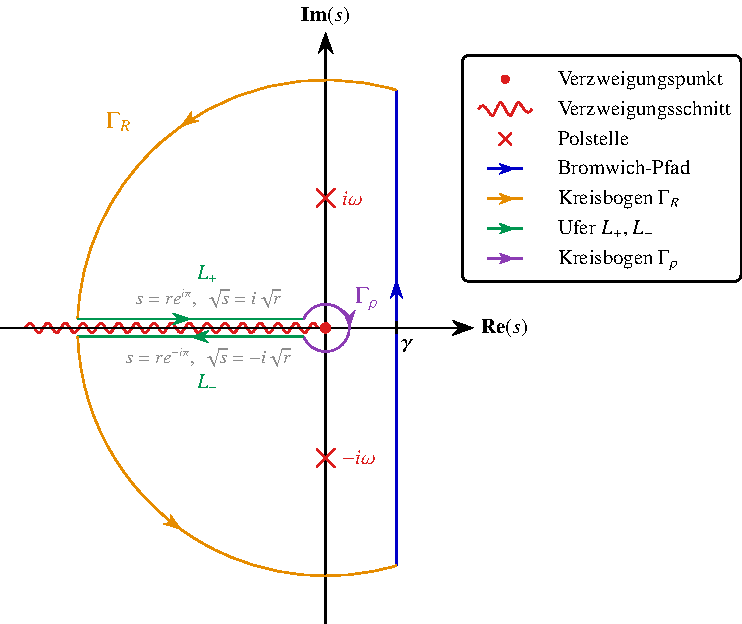
\includegraphics{papers/laplace/images/keyhole_kontur.pdf}
    \caption{Die Schlüsselloch-Kontur für Bildfunktionen mit
    Verzweigungspunkt bei $s = 0$.
    Der Verzweigungsschnitt (rote Wellenlinie) auf der negativen reellen
    Achse wird von den beiden horizontalen Wegen $L_+$ und $L_-$
    eingerahmt, der kleine Kreis $\Gamma_\rho$ umgeht den
    Verzweigungspunkt.
    Innerhalb der Kontur ist $\sqrt{s}$ eindeutig, und der Residuensatz
    erfasst nur die eingeschlossenen Pole, hier $s = \pm i\omega$.}
    \label{laplace:fig:keyhole_kontur}
\end{figure}
